\documentclass[aspectratio=169]{beamer}
\usepackage[english]{babel}
\usepackage[T1]{fontenc}
\usepackage{amsmath, amssymb, bm}
\usepackage{booktabs, xcolor}
\usepackage{tcolorbox}
\usepackage{graphicx}
\tcbuselibrary{skins}

\definecolor{primary}{RGB}{15, 45, 80}
\definecolor{secondary}{RGB}{0, 150, 136}
\usetheme{Madrid}
\usecolortheme{whale}
\setbeamercolor{structure}{fg=primary}
\setbeamercolor{title}{fg=white, bg=primary}
\setbeamercolor{block title}{bg=primary, fg=white}
\setbeamercolor{block body}{bg=primary!5, fg=black}
\setbeamertemplate{navigation symbols}{}
\setbeamertemplate{itemize items}[circle]
\newcommand{\hl}[1]{\textcolor{secondary}{\textbf{#1}}}

\title[EB-JEPA world model of drug perturbations]{An Energy-Based JEPA World Model of Drug Perturbations}
\subtitle{Predicting single-cell state in latent space on Tahoe-100M}
\author{Team Dynamics}
\institute{HackTheWorld(s) --- EB-JEPA}
\date{\today}

\begin{document}

\begin{frame}\titlepage\end{frame}

% ---------------- 1. PREMISE ----------------
\begin{frame}{The premise --- JEPA for cell biology}
\begin{block}{Predict, don't reconstruct}
Single-cell transcriptomes are \hl{noisy, sparse, high-dimensional sets} of genes.
Reconstructing counts (scGPT) is wasteful; \hl{predicting in a learned latent space}
(LeCun's JEPA) discards task-irrelevant noise. \emph{GeneJEPA} (Litman 2025) proved this on Tahoe-100M.
\end{block}
\begin{block}{Our goal}
A \hl{true Energy-Based JEPA \emph{world model}} of drug response ---
\hl{(control cell, drug) $\rightarrow$ perturbed cell} --- on a \hl{frozen pretrained encoder},
with \hl{biology-specific losses}, beating the standard baselines.
\end{block}
\end{frame}

% ---------------- 2. DATA composition ----------------
\begin{frame}{The data --- Tahoe-100M (Vevo/Arc): 100M cells, 1{,}000 lines, 3{,}000 drugs}
\centering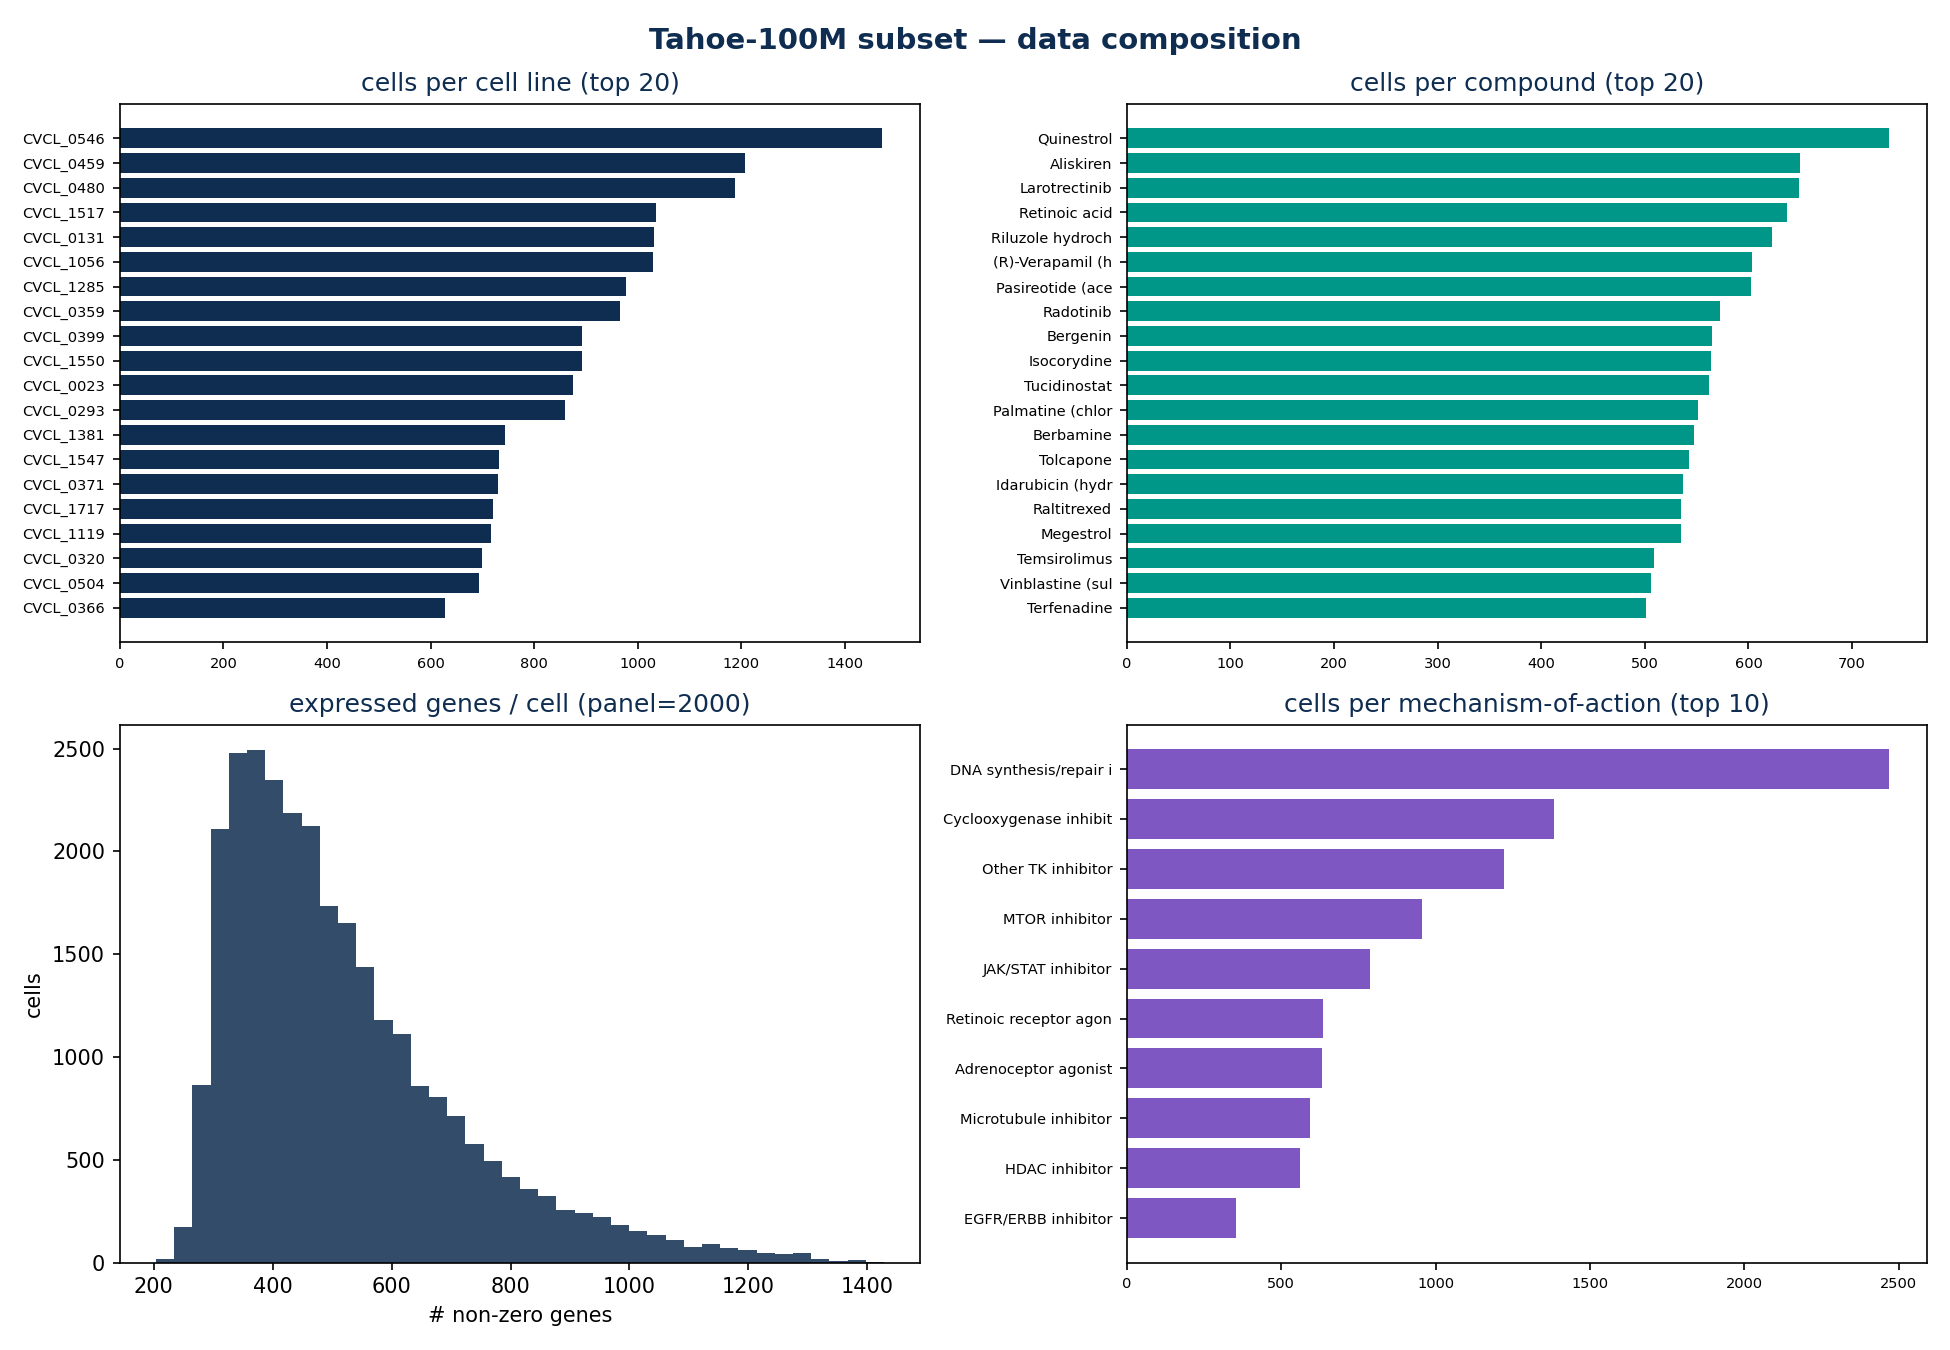
\includegraphics[height=0.66\textheight]{data_composition.png}\\
{\footnotesize Our subset: a Tahoe-x1 embeddings shard. Each cell = MosaicFM-3B embedding (2560-d)
$+$ drug $+$ cell line $+$ MoA. Preprocessing: top-K gene panel, per-feature z-score, co-expression modules.}
\end{frame}

% ---------------- 3. DATA umap ----------------
\begin{frame}{The data --- UMAP of the cell representations}
\centering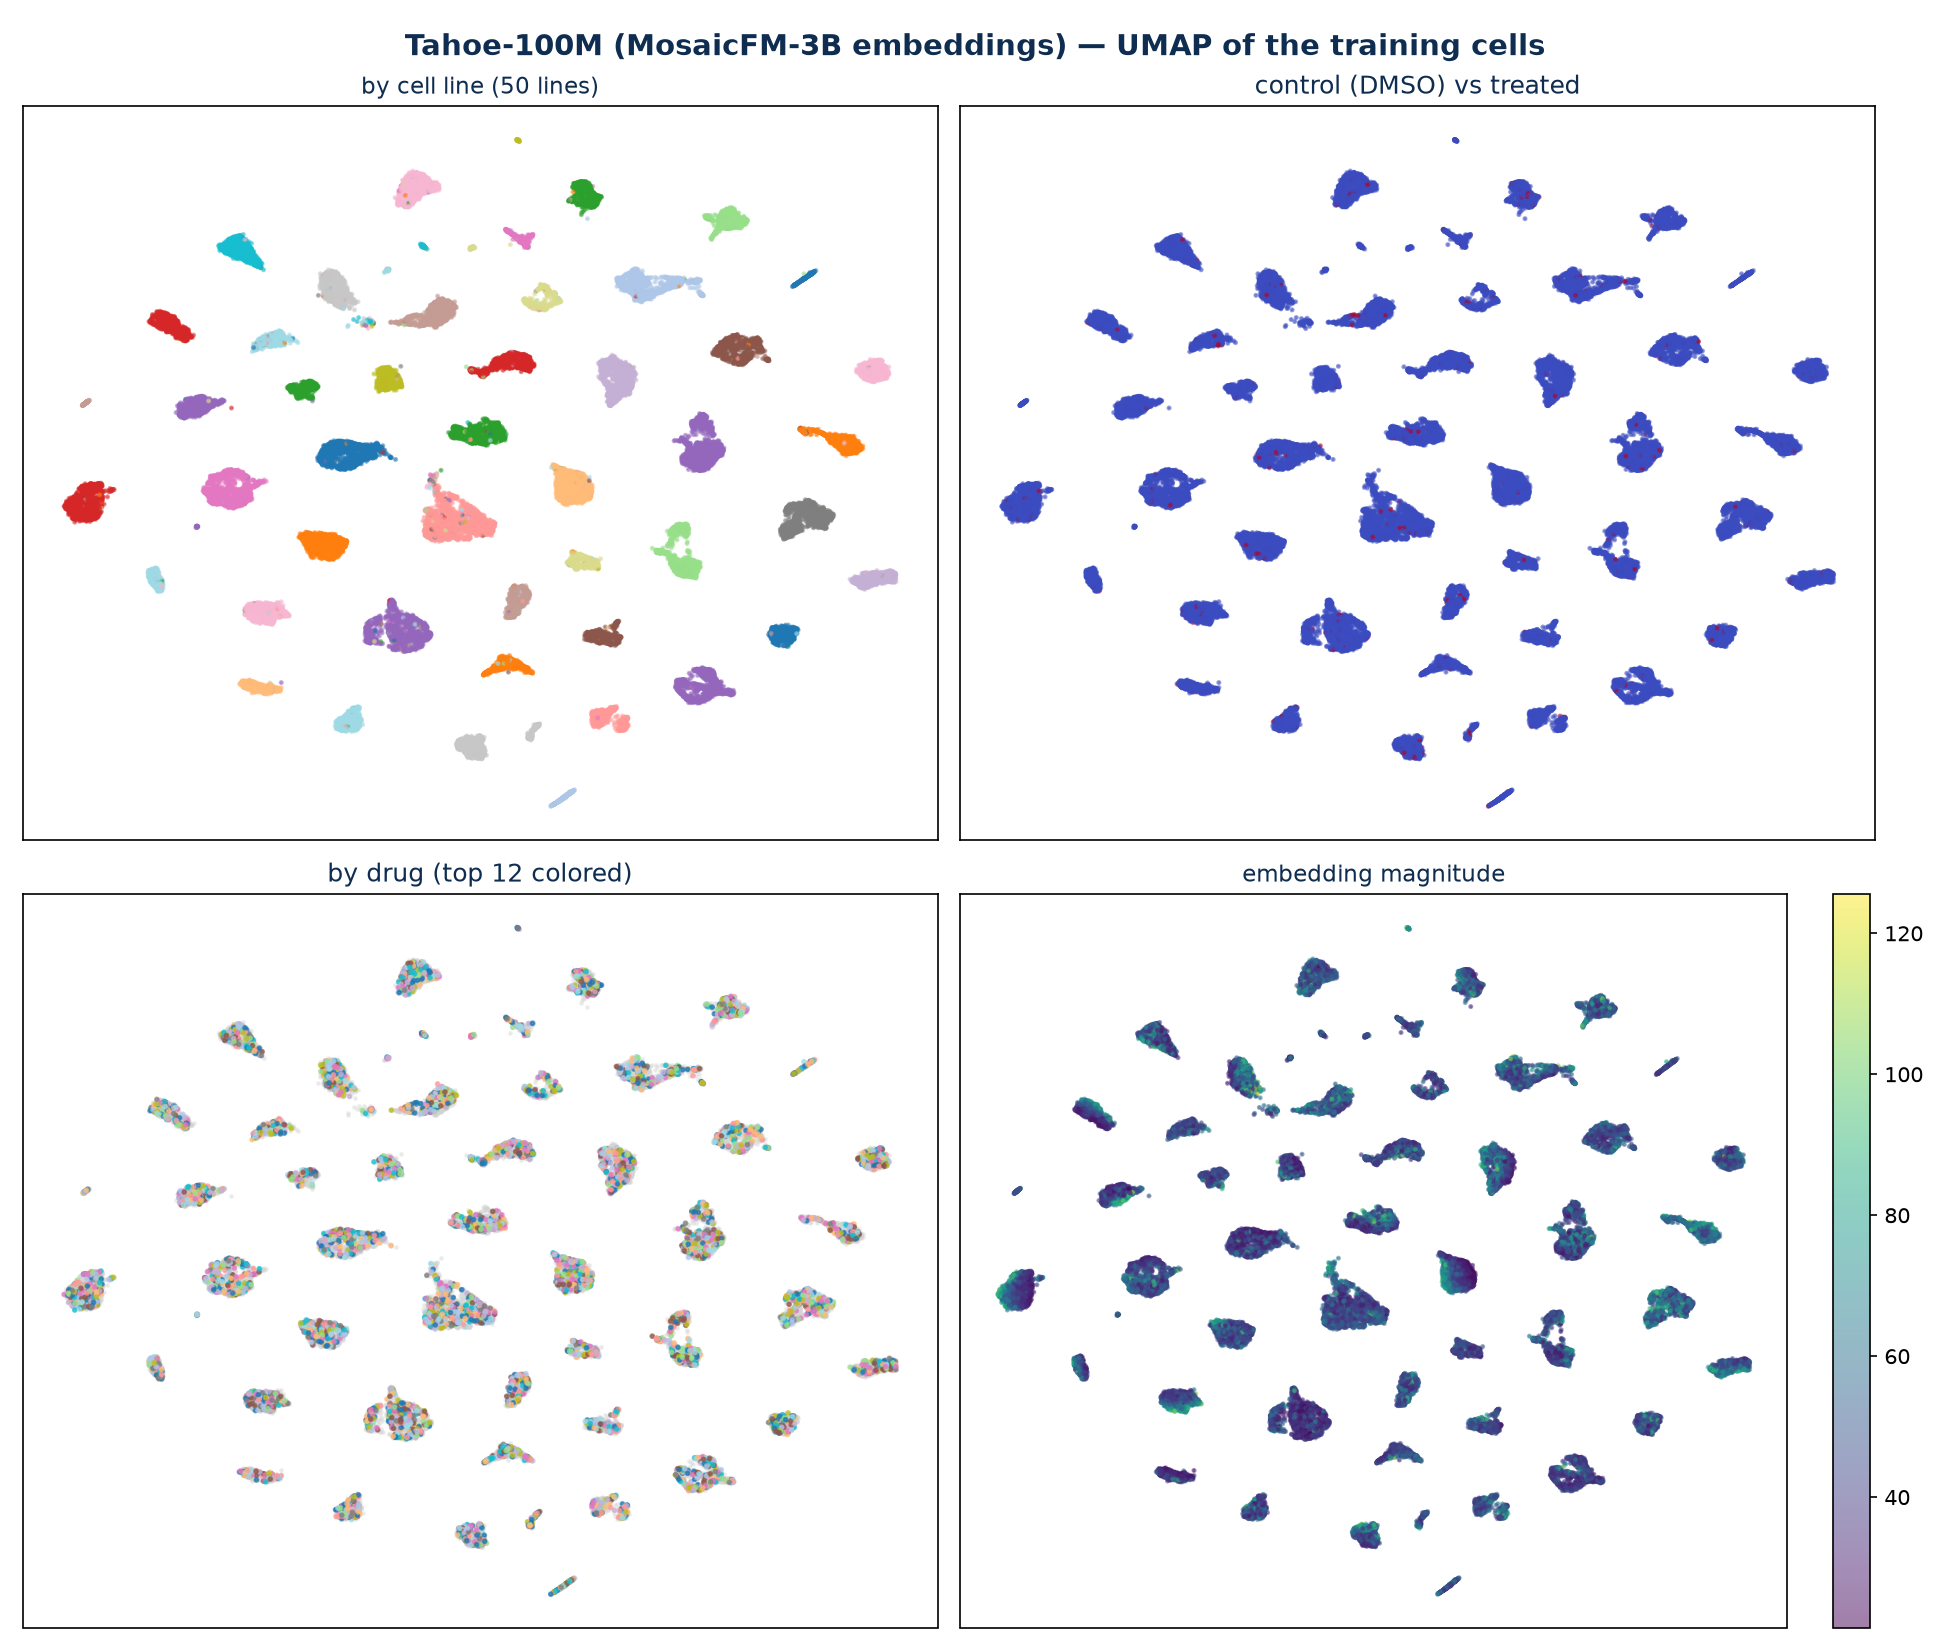
\includegraphics[height=0.70\textheight]{umap_panel.png}\\
{\footnotesize 40k cells. Clean structure by \hl{cell line}, a visible \hl{control vs treated} split,
and drug-level grouping --- a healthy space to build a world model on.}
\end{frame}

% ---------------- 4. RECIPE ----------------
\begin{frame}{The EB-JEPA recipe in one equation}
\begin{block}{Energy = prediction error in representation space}
\[ \mathcal{L} \;=\; \underbrace{\big\lVert g_\phi(f_\theta(x),\, q_\omega(a)) - f_\theta(x')\big\rVert^2}_{\text{predict target rep. from context + action}} \;+\; \lambda\, \mathcal{R}(z) \]
\end{block}
\small
\begin{itemize}
  \item \hl{$f_\theta$ encoder}, \hl{$g_\phi$ predictor}, \hl{$q_\omega$ action encoder}, \hl{$\mathcal{R}$ anti-collapse regularizer}.
  \item Three settings: image (identity $g_\phi$), video (predict next), \hl{action-conditioned (world model)} --- ours.
\end{itemize}
\end{frame}

% ---------------- 5. ARCHITECTURE ----------------
\begin{frame}{Our model --- frozen foundation encoder + learned drug predictor}
\begin{columns}
\begin{column}{0.58\textwidth}\small
\begin{itemize}
  \item \hl{$f_\theta$} = \textbf{frozen} MosaicFM-3B embedding (2560-d) --- a pretrained single-cell foundation encoder.
  \item \hl{$g_\phi$} = GRU predictor, \hl{conditioned on the drug} (action $a$).
  \item Energy $=\lVert g_\phi(z_{\text{ctrl}}, a) - z_{\text{pert}}\rVert^2$ via \texttt{eb\_jepa.JEPA.unroll}.
  \item \hl{Only the predictor is trained.} A drug is a \emph{large, controlled} state change $\Rightarrow$ \hl{no collapse} (unlike slow time series).
\end{itemize}
\end{column}
\begin{column}{0.42\textwidth}
\footnotesize
\begin{tcolorbox}[colback=secondary!8,colframe=primary,title={Pipeline}]
$z_{\text{ctrl}}$ (DMSO cell)\\
$\quad\downarrow\; g_\phi(\cdot,\ \text{drug})$\\
$\hat z_{\text{pert}}$\\
$\quad\downarrow$ energy vs real $z_{\text{pert}}$
\end{tcolorbox}
\end{column}
\end{columns}
\end{frame}

% ---------------- 6. CONTRIBUTIONS / LOSSES ----------------
\begin{frame}{Our contribution --- three biology-aware loss terms}
\small
\begin{tcolorbox}[colback=secondary!6,colframe=primary,title={1. SIGReg (anti-collapse; our choice vs GeneJEPA VICReg)}]
Forces the latent batch to be \hl{isotropic Gaussian} (Epps--Pulley statistic on random 1-D
projections). One hyper-parameter, linear cost, more stable than VICReg's two coefficients.
\end{tcolorbox}
\begin{tcolorbox}[colback=secondary!6,colframe=primary,title={2. PathwayCoherenceLoss (gene-program prior)}]
Latent pairwise distances must match \hl{co-expression-module activity} distances:
$\mathcal{L}_{\text{path}}=\lVert \widetilde{D}_{\text{latent}} - \widetilde{D}_{\text{module}}\rVert^2$. Injects biological program structure.
\end{tcolorbox}
\begin{tcolorbox}[colback=secondary!6,colframe=primary,title={3. PerturbationSignatureLoss (drug consistency)}]
Predicted shift $\hat z_{\text{pert}}-z_{\text{ctrl}}$ should point the \hl{same direction for the same drug}
(a compound has a characteristic signature) --- supervised-contrastive on shift directions.
\end{tcolorbox}
\end{frame}

% ---------------- 7. HEADLINE RESULT ----------------
\begin{frame}{Result --- the world model beats both baselines}
\begin{columns}
\begin{column}{0.5\textwidth}
\centering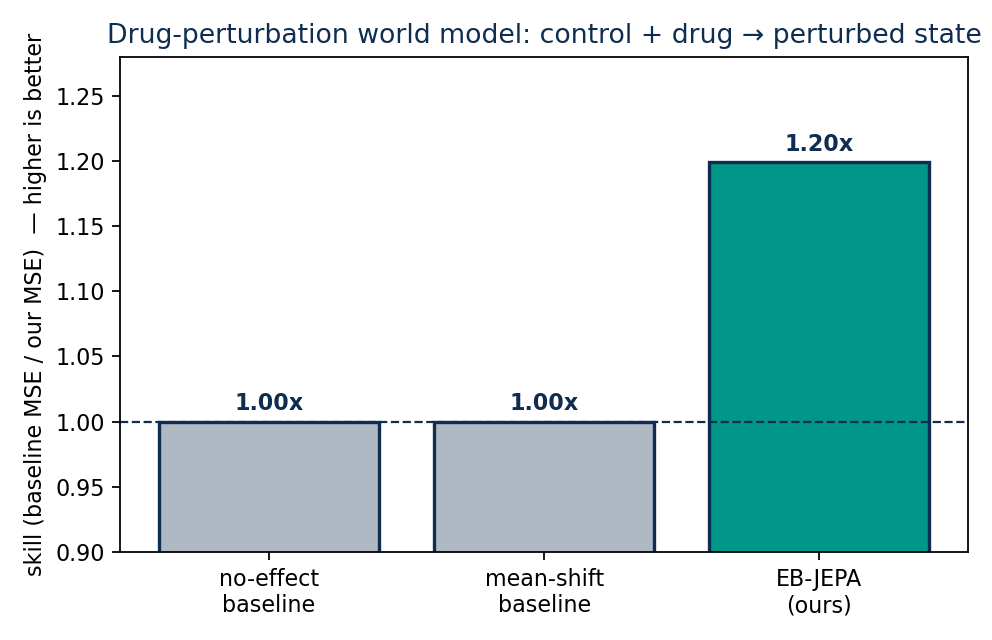
\includegraphics[width=\linewidth]{fig_skill.png}
\end{column}
\begin{column}{0.48\textwidth}\small
234k train / 59k val cells, real DMSO controls.
\begin{center}\footnotesize
\begin{tabular}{lc}
\toprule
predict $z_{\text{pert}}$ from\dots & rel. MSE $\downarrow$\\
\midrule
no-effect ($z_{\text{ctrl}}$) & 1.00\\
mean drug shift & 1.00\\
\hl{EB-JEPA (ours)} & \hl{0.83}\\
\bottomrule
\end{tabular}
\end{center}
\hl{skill 1.20$\times$ vs no-effect, 1.19$\times$ vs mean-shift.}
Beating \emph{mean-shift} = capturing \hl{context-specific} drug response.
\end{column}
\end{columns}
\end{frame}

% ---------------- 8. WHY WORLD MODEL ----------------
\begin{frame}{Why a world model? Plain SSL learns identity, not drugs}
\begin{columns}
\begin{column}{0.5\textwidth}\centering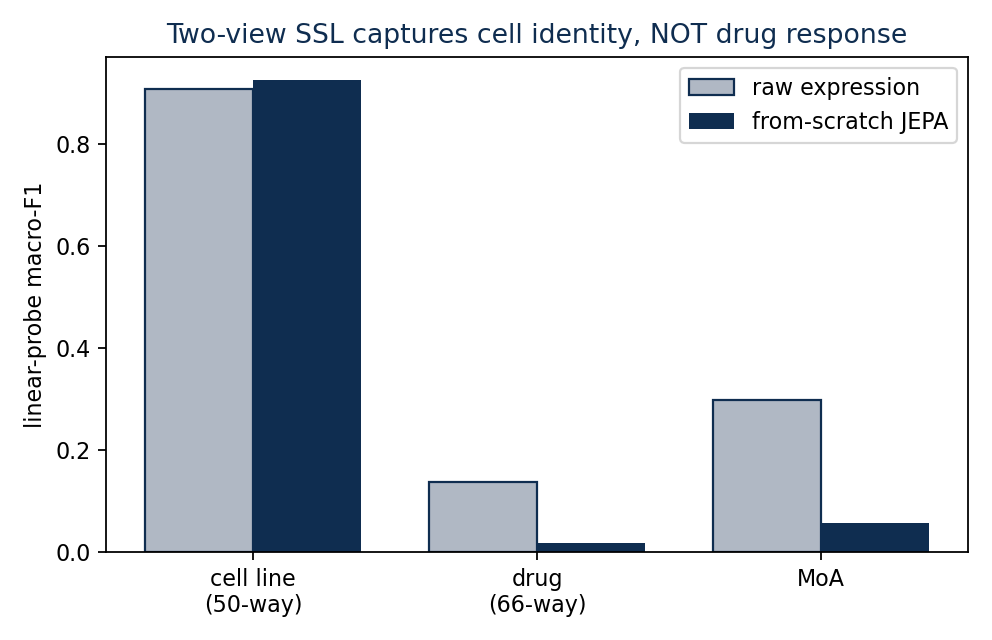
\includegraphics[width=\linewidth]{fig_probe.png}\end{column}
\begin{column}{0.48\textwidth}\small
A from-scratch two-view JEPA on raw genes (700k cells) linear-probes to
\hl{F1 0.93 on cell line} but \hl{0.02 on drug}.\\[4pt]
$\Rightarrow$ representation SSL organizes by the \hl{dominant variance (cell identity)};
\hl{drug response needs the action-conditioned predictor}.
\end{column}
\end{columns}
\end{frame}

% ---------------- 9. BENCHMARK ----------------
\begin{frame}{Benchmark --- PBMC3k cell type (literature dataset)}
\small
\begin{center}
\begin{tabular}{lcc}
\toprule
method & setting & macro-F1\\
\midrule
raw expression & in-domain & 0.94\\
PCA-50 & in-domain & 0.96\\
\hl{our cell JEPA} & in-domain & \hl{0.92}\\
\midrule
GeneJEPA & frozen transfer & 0.69\\
scGPT & frozen transfer & 0.23\\
\bottomrule
\end{tabular}
\end{center}
\hl{Honest read:} in-domain, raw expression is near-perfect on PBMC3k (cell types are
linearly separable) --- this benchmark does \emph{not} discriminate methods in-domain.
GeneJEPA's 0.69 is the much harder \emph{frozen-transfer} regime. \hl{Our edge is the
perturbation world model, where no trivial baseline exists.}
\end{frame}

% ---------------- 10. MICROBIOME finding ----------------
\begin{frame}{An honest negative --- microbiome dynamics collapse}
\begin{columns}
\begin{column}{0.5\textwidth}\centering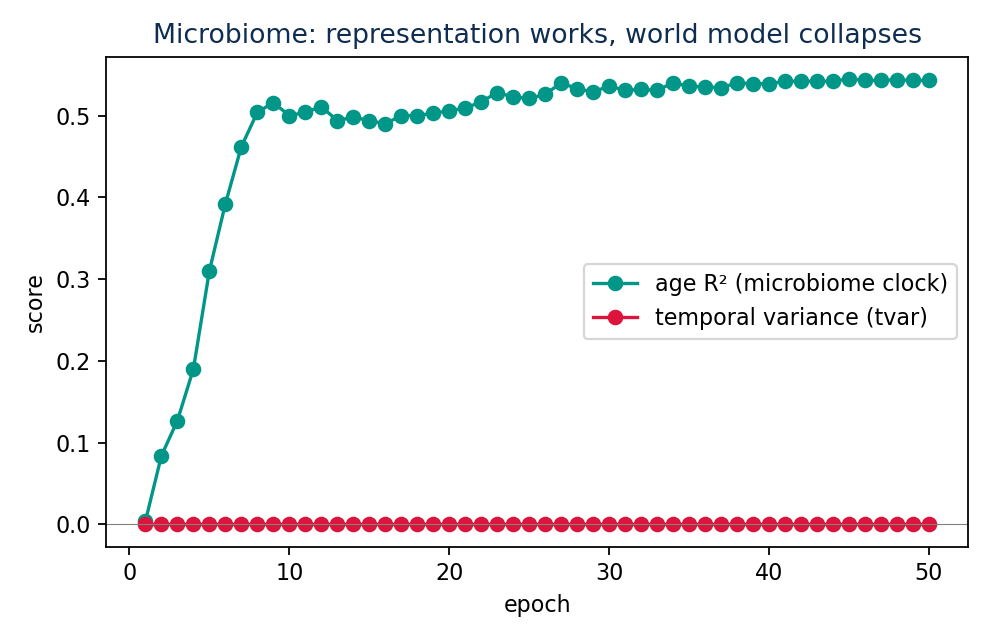
\includegraphics[width=\linewidth]{fig_microbiome.png}\end{column}
\begin{column}{0.48\textwidth}\small
Same recipe on DIABIMMUNE gut trajectories: representation works
(\hl{age $R^2\!\approx\!0.53$}, microbiome clock) but the world model
\hl{collapses temporally} (\texttt{tvar}$\to0$, skill $<1$).\\[4pt]
\hl{Insight:} VICReg keeps \emph{batch} variance, not \emph{temporal} variance ---
slow drift makes ``no change'' unbeatable. \hl{Controlled perturbations (Tahoe) remove the problem.}
\end{column}
\end{columns}
\end{frame}

% ---------------- 11. TAKEAWAYS ----------------
\begin{frame}{Takeaways}
\begin{block}{}
\begin{itemize}
  \item A \hl{true EB-JEPA world model} of drug perturbation (frozen MosaicFM + learned action predictor) that \hl{beats no-effect \& mean-shift baselines ($1.2\times$)} on Tahoe-100M.
  \item \hl{Three biology-aware design choices}: SIGReg, PathwayCoherenceLoss, PerturbationSignatureLoss --- our differentiators from GeneJEPA.
  \item A \hl{controlled, honest comparison} (+ a clean microbiome collapse finding that motivates the perturbation setting).
\end{itemize}
\end{block}
\centering\hl{Predict cellular response to drugs in latent space --- a step toward in-silico screening.}
\end{frame}

\end{document}
